% Conference paper; to be used with:
%         spconf.sty  - ICASSP/ICIP LaTeX style file, and
%         IEEEbib.bst - IEEE bibliography style file.
% --------------------------------------------------------------------------
\documentclass{article}
\usepackage{spconf,amsmath,graphicx,amssymb}
\usepackage{amsfonts}
\usepackage{amsthm}
\usepackage{booktabs}
\newtheorem{proposition}{Proposition}

% Custom math commands
\newcommand{\Rcomm}{R_{\text{comm}}}
\newcommand{\Rext}{R_{\text{ext}}}
\newcommand{\Rtotal}{R_{\text{total}}}
\newcommand{\VL}{V_L}
\newcommand{\AlphaRL}{\alpha_{\text{RL}}}
\newcommand{\AlphaRSA}{\alpha_{\text{RSA}}}
\newcommand{\Ltheta}{L_\theta}

% Title.
% ------
\title{Pragmatic Rewards: Intrinsic Communicative Clarity\\ in Multi-Agent Reinforcement Learning}
%
% Single address.
% ---------------
\name{Henri Langlois, Pablo Piantanida}
\address{CNRS, ILLS, Mila, CentraleSup\'elec}

\begin{document}
\maketitle
%
\begin{abstract}
Reinforcement Learning (RL) agents often fail in cooperative settings because their actions, while individually optimal, are unpredictable to their partners. This challenge is magnified in human-agent teams, where an agent's opacity can erode trust and team effectiveness. We address this limitation by establishing a formal equivalence between pragmatic inference, as formalized by the Rational Speech Act (RSA) framework, and Maximum Entropy Reinforcement Learning (Max-Ent RL). This theoretical bridge yields a principled intrinsic reward for ``legible'' behavior---actions that clearly communicate an agent's private state---computed offline by a Pragmatic Reward Module (PRM) that adds no latency to decision-making. The framework exposes the \emph{literal listener} $L_0$, the assumed common ground against which clarity is measured, as its central design choice. We study a spectrum of listeners, from hand-crafted geometric heuristics to a listener \emph{learned} jointly with the policy, and show that the learned instantiation turns the pragmatic reward into a variational lower bound on the mutual information between an agent's intention and its observable behavior, unifying pragmatic and information-theoretic approaches to implicit communication. We evaluate on two environments separated by an \emph{oracle-gap} criterion that bounds the task value of communication: a cooperative-navigation control where the gap is near zero, and \emph{scout-support}, a new tractable benchmark modeled on pickup-and-delivery teams in which a scout's private target only pays off if a slower teammate infers it early. The experiments dissect implicit communication into its two sides. On the speaker side, hand-crafted listeners range from \emph{miscalibrated signaling}---costly behavior whose own intrinsic reward stays below the uninformative level---to calibrated designs, while the learned listener renders behavior decodable at 92\%. On the receiver side, no reward-trained teammate learns to read any of it; deploying the learned listener as the teammate's ``ear'' at execution recovers part of the gap. What remains is a two-sided coordination equilibrium in which uniformly-integrated clarity rewards buy \emph{lazy} clarity---informative where it is cheap, silent where the partner needs it---which we argue redirects the design problem for legibility rewards from \emph{how much} to \emph{when}. Our framework provides a formal model, a benchmark, and a diagnosis for agents that are not only effective but also strategically collaborative.
\end{abstract}
%
\begin{keywords}
Reinforcement Learning, Intrinsic Motivation, Multi-Agent Systems, Computational Pragmatics, Legibility
\end{keywords}
%
\section{Introduction}
\label{sec:intro}

Human collaboration is fundamentally a goal-oriented, strategic activity. To succeed, we do not just act to achieve our own goals; we act in ways that allow our partners to infer our beliefs and intentions, enabling better coordination. The same is true for artificial agents. In cooperative multi-agent reinforcement learning (MARL) environments, an agent's success depends not only on its own actions but also on being understood by its teammates. Consider a cooperative navigation task in which each agent must cover a target of a preferred type: an agent that simply rushes toward its target may take a path that is ambiguous from a teammate's perspective, causing the teammate to abandon a target the agent never intended to claim. A more sophisticated agent might take a slightly suboptimal path that unambiguously singles out its intended target, making its intention clear and enabling better team coordination.

This property of being easily understood is called ``legibility'' \cite{dragan2013legibility}. However, standard RL agents, optimized solely for an extrinsic task reward, have no incentive to be legible. This leads to our central question: how can we formally encourage an RL agent to choose actions that are not just extrinsically optimal for the task, but also intrinsically optimal for communicating its private state or intentions?

This work proposes a solution in the form of an intrinsic reward, $\Rcomm$, that quantifies the communicative clarity of an agent's actions. To calculate this reward, we model an ``observer'' (e.g., another agent) who uses pragmatic inference to reason about \emph{why} the agent chose a particular action over the available alternatives. We find the ideal formalism for this observer in the Rational Speech Act (RSA) framework \cite{goodman2016pragmatic}, which provides a formal account of reasoning about communicative intent.

Any such observer model must be anchored in a \emph{literal listener} $L_0$: the assumed common ground that specifies how behavior would be interpreted in the absence of pragmatic reasoning. Our analysis and experiments show that this choice is not an implementation detail but the decisive factor in whether pragmatic rewards help or hurt. Hand-crafted listeners can be systematically misaligned with what the policy can express, incentivizing \emph{costly signaling} that an actual observer cannot decode. This motivates our second contribution: replacing the hand-crafted $L_0$ with a listener learned from the agents' own behavior, which guarantees, by construction, that rewarded actions are decodable.

Our contributions are as follows:
\begin{itemize}
\item We establish a formal equivalence between the objective functions of Max-Ent RL and the RSA framework, allowing the RSA ``listener value'' to be imported as a principled intrinsic reward for legibility, and we show that purely communicative models such as CRSA \cite{estienne2025collaborative} are recovered as a myopic special case ($\gamma=0$, $\Rext=0$).
\item We operationalize the theory as a \emph{Pragmatic Reward Module} (PRM): an offline component, compatible with centralized training and decentralized execution (CTDE), that computes $\Rcomm$ from replayed transitions and adds no latency at execution time.
\item We characterize the space of literal listeners and prove that instantiating $L_0$ with a listener trained by maximum likelihood on the agents' behavior makes the expected pragmatic reward a variational lower bound on the mutual information $I(M; S, A)$ between private intentions and observable behavior. This connects pragmatic rewards to information-regularization \cite{strouse2018learning} and skill-discriminability \cite{eysenbach2019diversity} objectives, and positions them as the \emph{literal} (0-th order) special case of our framework.
\item We propose an \emph{oracle-gap} criterion for benchmarking communicative rewards---the gap between a baseline and an oracle given all private states bounds the task value of communication---and introduce \emph{scout-support}, a tractable two-agent benchmark with a large, structural gap: a scout's private target only pays off if a slower supporter infers it early, while a pickup waypoint makes the scout's task-optimal motion uninformative exactly when information is needed. A cooperative-navigation control with near-zero gap completes the pair.
\item Empirically, we dissect implicit communication into speaker and receiver contributions. Hand-crafted listeners range from \emph{miscalibrated signaling} (intrinsic reward stuck below the uninformative level, task cost up to 47\% in the control) to well-calibrated progress- and filter-based designs; yet no speaker-side reward alone moves the teammate's understanding. The learned listener proves the channel exists---decoding the speaker at $92\%$---and deploying it as the teammate's \emph{ear} at execution recovers part of the oracle gap, isolating a joint-exploration equilibrium, not legibility, as the remaining obstacle.
\end{itemize}

\section{Related Work}
\label{sec:related}

Our framework, which uses pragmatic inference to generate an intrinsic reward for communicative clarity, builds on four lines of research: (1) legibility and observer-aware planning; (2) intrinsic rewards for multi-agent coordination; (3) implicit and emergent communication; and (4) computational pragmatics.

\subsection{Legibility, Goal Recognition, and Observer-Aware Planning}

Inferring an agent's latent state (e.g., its goal) from observed behavior is the central problem of Inverse Reinforcement Learning (IRL) \cite{ziebart2008maximum} and computational Theory of Mind (ToM) \cite{baker2017rational,rabinowitz2018machine}. Legibility inverts this problem: the actor shapes its own behavior so that an observer's inference succeeds. Originally formalized for robot motion \cite{dragan2013legibility}, legibility has been extended to stochastic sequential decision problems \cite{faria2024guess}, unified with explicability and predictability in observer-aware MDPs \cite{miura2021unifying,miura2024observer}, and recently brought to MARL through legible variants of interactive POMDPs \cite{liu2025active}. These approaches typically embed the observer model in the \emph{planning} objective, requiring inference over goals at decision time. In contrast, our framework converts legibility into an \emph{intrinsic reward} computed offline during training, so the executed policy carries its communicative competence ``for free,'' with no observer model, belief tracking, or additional computation in the execution loop.

A complementary line of work uses ToM as a source of intrinsic motivation \cite{oguntola2023theory}, rewarding agents for accurately predicting the beliefs of others; this is listener-centric, rewarding agents for being predictive of others. Our pragmatic framework is speaker-centric: it rewards agents for making their own private state clear, regardless of their partners' modeling ability.

\subsection{Intrinsic Rewards for Multi-Agent Coordination}

Our pragmatic reward is a form of intrinsic motivation for cooperation, and is thus related to social influence \cite{jaques2019social}, which rewards an agent for causally changing its partners' behavior. The communicative goals differ: influence rewards an agent for \emph{compelling} a reaction, whereas the pragmatic reward incentivizes the successful \emph{transmission} of information about oneself, decoupling the speaker's reward from the listener's reaction. Teammates remain free to exploit or ignore the revealed intention, which promotes a more flexible form of coordination.

Closest to our learned-listener instantiation is the information-regularization framework of Strouse et al.~\cite{strouse2018learning}, which adds a mutual-information term $I(A;G|S)$ to the objective so that agents share (or hide) their goal $G$ through their actions. Similarly, Eccles et al.~\cite{eccles2019biases} add a positive-signaling bias encouraging messages to depend informatively on observations, and, in the single-agent setting, DIAYN \cite{eysenbach2019diversity} rewards skills for being discriminable from states via a learned classifier. Proposition~\ref{prop:mi} makes the relationship precise: these MI-based objectives correspond to the \emph{literal} listener level of our framework, obtained when the RSA recursion depth is zero and $L_0$ is trained by maximum likelihood. The pragmatic levels add contrastive reasoning over the alternative actions the agent could have taken---a model of communication richer than statistical dependence alone. Our framework also shares the goal of grounded, convention-free coordination with Bayesian action decoding \cite{bard} and off-belief learning \cite{obl}, which control how much agents may read into their partners' actions; we instead directly reward the actor for making the intended reading easy.

\subsection{Implicit Communication vs.\ Explicit Channels}

A significant body of MARL research equips agents with a dedicated communication channel and learns an emergent protocol end-to-end \cite{foerster2016learning,sukhbaatar2016learning,boldt2024review}. Our framework diverges from this paradigm by focusing on \emph{implicit} communication: there is no separate channel and no explicit message passing. An agent ``speaks'' by moving in the environment, and a teammate ``listens'' by observing that movement. The pragmatic reward incentivizes actions that are simultaneously effective for the task and clear as signals of intent. This is valuable when explicit communication is costly, unavailable, or must be fused with physical action, as is common in human-agent teams. Because the signal \emph{is} the action, the exploration-communication conflict identified in emergent-communication work \cite{eccles2019biases,sad} appears here as a reward-shaping trade-off, which we analyze through the weight $\lambda$.

\subsection{Computational Pragmatics}

RSA \cite{goodman2016pragmatic} formalizes communication as recursive probabilistic reasoning between a speaker and a listener, and has been given a rate-distortion interpretation \cite{zaslavsky2021rate}. Neural instantiations replace the hand-specified literal listener with learned models \cite{andreas2016reasoning,fried2018unified}, a design choice our learned-$\Ltheta$ instantiation transposes to the behavioral domain. The Collaborative RSA (CRSA) model \cite{estienne2025collaborative} extends RSA to multi-turn dialog between agents with asymmetric private information. We show in Section~\ref{ssec:recover_crsa} that such purely communicative models arise as the myopic, task-free special case of our strategic framework, which extends pragmatic reasoning to long-horizon sequential decision-making where instrumental and communicative goals are intertwined.

\section{Formalisms for Action and Interpretation}
\label{sec:background}

To model legible strategic behavior we require two formalisms: one for optimal sequential decision-making under uncertainty, and one for how an observer infers intent from an action. For the former we use Max-Ent RL; for the latter, RSA.

\subsection{Maximum Entropy RL}
\label{ssec:maxentrl}

Max-Ent RL extends the standard RL objective with the intuition ``be as versatile as possible while still being successful.'' In a single-step problem, the agent seeks a policy $\pi(a|s)$ maximizing expected reward plus policy entropy \cite{haarnoja2018soft}:
\begin{equation}
J(\pi)=\mathbb{E}_{a\sim\pi(\cdot|s)}[R(s,a)]+\AlphaRL H(\pi(\cdot|s)).
\end{equation}
The optimal policy is a softmax over rewards \cite{levine2018reinforcement}, with temperature $\AlphaRL$ trading off exploitation against versatility:
\begin{equation}
\pi^{*}(a|s)\propto \exp\left(R(s,a)/\AlphaRL\right). \label{eq:maxent_policy}
\end{equation}

\subsection{The Rational Speech Act Framework}
\label{ssec:rsa}

RSA \cite{goodman2016pragmatic} models an observer who infers an agent's intended meaning not from the literal content of an action alone, but by reasoning about why the agent chose that action over the alternatives: ``if they had intended $X$, they would have done $Y$; since they did $Z$, they must intend something else.'' Formally, RSA seeks a communicative policy $S(u|m)$ that optimally balances communicative success against action cost, yielding a softmax over the utility, or ``listener value,'' of each communicative act:
\begin{equation}
S(u|m)\propto \exp(\AlphaRSA\cdot \VL(u,m)), \label{eq:rsa_policy}
\end{equation}
where $\VL(u,m)$ quantifies the clarity of act $u$ for conveying meaning $m$ to an observer, penalized by the act's cost.

\section{Rewarding Legibility}
\label{sec:pragmatic_reward}

Our agent optimizes a composite reward balancing task objectives with communicative clarity. This section defines the reward via a formal bridge between pragmatic inference and RL, characterizes the space of listener models that anchor it, describes the architecture that computes it, and presents the resulting strategic Bellman equation.

\subsection{The Total Reward}
\label{ssec:total_reward}

At each timestep $t$ the agent receives the standard \textbf{extrinsic task reward} $\Rext(s_t,a_t)$ from the environment, and generates internally an \textbf{intrinsic communicative reward} $\Rcomm(s_t,a_t)$ quantifying how clearly action $a_t$ communicates the agent's private state $m_t$ (its ``meaning,'' e.g., an intended target) to an imagined observer. The policy maximizes the weighted sum
\begin{equation}
\Rtotal(s_t, a_t) = \Rext(s_t, a_t) + \lambda\, \Rcomm(s_t, a_t), \label{eq:total_reward}
\end{equation}
where $\lambda$ balances task success against communicative clarity. The central question is how to define $\Rcomm$ in a principled way.

\subsection{Deriving $\Rcomm$ via Pragmatic Inference}
\label{ssec:reward_derivation}

We treat the agent's action $a$ as a communicative ``utterance'' and its private state $m$ as the ``meaning'' to be conveyed (Table~\ref{tab:mapping}). At first glance, the objective of an RL agent and the goal of a pragmatic speaker seem unrelated. However, the optimal single-step Max-Ent policy (Eq.~\ref{eq:maxent_policy}) and the RSA speaker (Eq.~\ref{eq:rsa_policy}) are both softmax distributions, identical under the re-indexing $\AlphaRSA = 1/\AlphaRL$. This formal alignment is the cornerstone of our framework: it justifies importing the well-defined listener value $\VL$ from computational pragmatics as a principled intrinsic reward. We define
\begin{equation}
\Rcomm(s_t, a_t) \triangleq \VL(a_t, m_t) = \log L^*_t(m_t|a_t, s_t) - C(a_t), \label{eq:comm_reward_def}
\end{equation}
where $L^*_t(m_t|a_t,s_t)$ is the probability a pragmatic listener assigns to the agent's true private state after observing its action in context $s_t$, and $C(a_t)$ is an optional action cost. In practice we set $C(a_t)=0$: the cost of a legible action is already handled by the task reward, since a less direct but clearer path is naturally penalized by a lower $\Rext$. In our implementation we also add the constant $\log|\mathcal{M}|$, so that $\Rcomm$ reads as the \emph{information gain} over a uniform prior: it is zero when the action is uninformative and positive when the listener's posterior concentrates on the true meaning.

\begin{table}[t]
\centering
\caption{Mapping between Max-Ent RL and RSA components.}
\label{tab:mapping}
\begin{tabular}{ll}
\toprule
\textbf{Max-Ent RL component} & \textbf{RSA analogue} \\
\midrule
State ($s$) & Context \\
Action ($a$) & Utterance ($u$) \\
Private state / intention ($m$) & Meaning ($m$) \\
Agent policy ($\pi(a|s,m)$) & Speaker ($S(u|m)$) \\
Intrinsic reward ($\Rcomm$) & Listener value ($\VL$) \\
Temperature ($\AlphaRL$) & Rationality ($1/\AlphaRSA$) \\
\bottomrule
\end{tabular}
\end{table}

\subsection{The Space of Literal Listeners}
\label{ssec:listeners}

Computing $L^*$ requires anchoring the pragmatic recursion in a \emph{literal listener} $L_0(m|a,s)$: the assumed common ground specifying how behavior would be interpreted absent pragmatic reasoning. Given $L_0$ and a set $\mathcal{A}$ of alternative actions (the true action plus $K$ sampled alternatives), the pragmatic listener is obtained by $N_r$ steps of RSA alternation,
\begin{equation}
S_k(a|m) = \frac{L_{k-1}(m|a)}{\sum\limits_{a'\in\mathcal{A}} L_{k-1}(m|a')}, \;\;
L_k(m|a) = \frac{S_k(a|m)}{\sum\limits_{m'} S_k(a|m')}, \label{eq:rsa_recursion}
\end{equation}
and $L^* = L_{N_r}$. The choice of $L_0$ is the framework's most consequential free parameter, and we study three instantiations.

\textbf{(i) Direction listeners.} A computationally cheap heuristic interprets actions by their geometric similarity to ideal paths. For agent position $p$ and each meaning $m$, let $v_m$ be the unit vector toward the nearest target consistent with $m$. A na\"ive score is $S(a,m) = \alpha_{\text{temp}}\cos(a, v_m)$ (\emph{simple}). To capture unambiguity explicitly, an \emph{exclusivity} variant penalizes similarity to competing meanings,
\begin{equation}
S_{\text{excl}}(a, m) = \alpha_{\text{temp}} \big( \cos(a, v_m) - \max_{m' \neq m} \cos(a, v_{m'}) \big), \label{eq:exclusivity}
\end{equation}
and $L_0(\cdot|a) = \mathrm{softmax}_m\, S_{\text{excl}}(a,\cdot)$. This listener rewards actions aligned with the ideal path toward the true target \emph{and} misaligned with the ideal paths of all confusable targets.

\textbf{(ii) Progress listener.} Instead of instantaneous direction, this listener scores the \emph{progress} an action realizes toward each candidate target: $S_{\text{prog}}(a,m) \propto d_{t-1}(m) - d_t(m)$, the per-step reduction in distance to the target consistent with $m$, normalized by the maximum step length. This mirrors the cost-to-go formulation of legibility in robot motion \cite{dragan2013legibility}, which scores partial trajectories by how efficiently they advance each candidate goal.

\textbf{(iii) Filter listener.} Instantaneous listeners ignore history: an action that is uninformative in isolation may complete a legible trajectory. The filter listener maintains a recursive belief over meanings, updated multiplicatively from per-step directional likelihoods with exponential forgetting,
\begin{equation}
b_t(m) \propto b_{t-1}(m)^{\rho}\, \exp\!\big(\alpha_{\text{temp}} \cos(a_t, v_m)\big), \label{eq:filter}
\end{equation}
and rewards the log-belief in the true meaning, $\Rcomm = \log b_t(m_t) + \log|\mathcal{M}|$. Under discounting this reproduces the trajectory-integral character of legibility---early clarity is worth more than late clarity---and makes $\Rcomm$ explicitly non-Markovian, which the PRM accommodates because rewards are computed offline.

\textbf{(iv) Learned listener.} Hand-crafted listeners presuppose that the features they score are the ones an actual observer would use. To remove this assumption, we train a network $\Ltheta(m|s,a)$ by maximum likelihood on the replay buffer to predict an agent's true meaning from its publicly observable context and action (the private state is masked from the input). The listener is trained concurrently with the policy, so the common ground \emph{co-adapts}: the reward only credits signals that are actually decodable from the agents' current behavioral distribution. With $N_r=0$ the reward is simply $\Rcomm = \log \Ltheta(m_t|s_t,a_t) + \log|\mathcal{M}|$; with $N_r\geq 1$ the RSA recursion (Eq.~\ref{eq:rsa_recursion}) is applied on top of $\Ltheta$, adding contrastive reasoning over alternatives.

The learned instantiation admits an information-theoretic characterization.

\begin{proposition}
\label{prop:mi}
Let meanings be drawn uniformly on $\mathcal{M}$, and let $\Ltheta(m|s,a)$ be any conditional distribution. Then, under the joint distribution induced by the policy,
\begin{equation}
\mathbb{E}\big[\log \Ltheta(m|s_t,a_t) + \log|\mathcal{M}|\big] \;\leq\; I(M; S_t, A_t),
\end{equation}
with equality iff $\Ltheta(m|s,a) = p(m|s_t=s, a_t=a)$. Hence the expected learned-listener reward is the Barber--Agakov variational lower bound \cite{barber2003im} on the mutual information between the agent's private meaning and its observable behavior; maximum-likelihood training of $\theta$ tightens the bound, and policy optimization against it maximizes information disclosure.
\end{proposition}

\begin{proof}
$\mathbb{E}[\log \Ltheta(m|s,a)] = \mathbb{E}[\log p(m|s,a)] - \mathbb{E}_{s,a}\big[\mathrm{KL}(p(\cdot|s,a)\,\|\,\Ltheta(\cdot|s,a))\big] \leq -H(M|S_t,A_t)$. Adding $H(M) = \log|\mathcal{M}|$ gives the claim; the KL term vanishes iff $\Ltheta$ matches the true posterior.
\end{proof}

Proposition~\ref{prop:mi} unifies two families of methods. The cooperative information regularizer of Strouse et al.~\cite{strouse2018learning}, the positive-signaling bias of Eccles et al.~\cite{eccles2019biases}, and the skill discriminator of DIAYN \cite{eysenbach2019diversity} all maximize variational MI bounds of exactly this form; within our framework they are the \emph{literal} ($N_r=0$) level of pragmatic reasoning with a learned common ground. Conversely, the RSA recursion is a strict generalization that scores an action not by how much information it carries in isolation, but by how it contrasts with the alternatives the agent declined---the signature of pragmatic communication \cite{goodman2016pragmatic,zaslavsky2021rate}.

\subsection{The Pragmatic Reward Module}
\label{ssec:architecture}

The theoretical bridge yields a practical hybrid architecture that decouples action selection from communicative analysis. The system comprises the main RL agent, which learns $\pi(a_t|s_t)$, and a \emph{Pragmatic Reward Module} (PRM), which computes $\Rcomm$ to shape the agent's learning updates. The pragmatic analysis is performed \emph{offline} during training---for static listeners, when a transition is collected; for the learned listener, when it is replayed, so the reward tracks the co-adapting common ground---and never in the action-selection loop, adding no latency to decision-making. We operate under CTDE: during centralized training the PRM has access to all agents' private states, enabling a gold-standard legibility reward; at execution, agents act from local observations only, and the PRM is discarded.

\subsection{The Strategic Bellman Equation}
\label{ssec:bellman}

With the composite reward defined, the action-value function of the legible agent satisfies the soft Bellman equation
\begin{equation}
\label{eq:full_bellman}
\begin{split}
    Q_t(s_t, a_t) ={}& \Rtotal(s_t, a_t) \,+ \\
                     & \gamma\, \mathbb{E}_{s_{t+1}}\Big[\alpha \log \sum_{a_{t+1}} \exp\big(\tfrac{1}{\alpha}Q_{t+1}(s_{t+1}, a_{t+1})\big)\Big],
\end{split}
\end{equation}
which is the standard Max-Ent backup applied to $\Rtotal$. The equation makes explicit the trade-off between immediate gains (task and clarity) and the long-term strategic value of future states: an agent may accept a lower immediate reward (e.g., a ``corralling'' detour) if the resulting state carries higher expected value through improved team coordination.

\subsection{Generality: Recovering Communicative Agents}
\label{ssec:recover_crsa}

Purely communicative agents arise as a special case. Setting $\Rext=0$ and $\lambda=1$ makes the total reward purely communicative; setting $\gamma=0$ makes the agent myopic, collapsing Eq.~\ref{eq:full_bellman} to the immediate reward plus policy entropy. This objective is exactly the per-turn gain function of the Collaborative RSA model \cite{estienne2025collaborative}, demonstrating that single-turn pragmatic models are a specific instance of our framework, which extends pragmatic reasoning to long-horizon sequential settings where instrumental and communicative goals interact.

\section{Experimental Setup}
\label{sec:methodology}

\subsection{Environments}
\label{ssec:environments}

A meaningful benchmark for communicative rewards must certify that communication has task value at all. We therefore adopt an \emph{oracle-gap} criterion: comparing a baseline against an oracle that receives all private states in its observations measures the maximum task reward that intent transmission can unlock. We evaluate on two environments, one on each side of this criterion.

\textbf{Environment A: scout-support (oracle gap $\approx 0.5$ per step).} A two-agent team in a continuous 2D arena, modeled on scout-and-support patterns in search-and-rescue and warehouse logistics: a fast \emph{scout} privately knows which of three sites is the true target, and a slower \emph{supporter} earns the team a bonus only while both agents occupy the target together. Crucially, the scout must first visit a central \emph{pickup waypoint} before its presence at the target counts (a forklift fetches the pallet before the dock). During this first leg, the scout's task-optimal motion is identical regardless of target---structurally uninformative---so any early information the supporter receives must be actively signaled, e.g.\ by curving the approach to the waypoint toward the future destination, the anticipatory motion studied in robot legibility \cite{dragan2013legibility}. Sites lie on a circle (radius $1.0$, $120^\circ$ apart, jittered); the supporter's lower speed ($0.6$ vs.\ $1.0$) makes late commitment costly. The reward is the rendezvous bonus minus both agents' distances to their current objectives; episodes last 50 steps. The supporter observes the scout's position and velocity but never its target. Meanings are the three sites; only the scout receives $\Rcomm$.

\textbf{Environment B: preference spread (oracle gap $\approx 0$).} Our earlier cooperative-navigation control: three agents and three colored landmarks, each agent holding a private color preference; the team is rewarded for matched coverage, penalized for distance and collisions. Because proximity resolves most coordination and acting on one's own preference is extrinsically rewarded, an oracle gains nothing---communication here has no task value to unlock, which is precisely what makes it a useful control for measuring what a communicative reward \emph{costs}.

\subsection{Models and Conditions}
\label{ssec:models}

All agents are trained with multi-agent Soft Actor-Critic (MASAC)---parameter-shared Gaussian actors (roles distinguished by a one-hot flag) and a centralized twin critic over joint observations and actions, with automatic entropy tuning---the natural multi-agent extension of the Max-Ent framework our theory is built on. Conditions differ only in reward and observation content: \textbf{baseline} ($\lambda=0$); \textbf{oracle} ($\lambda=0$, private states shared through observations); the four hand-crafted listeners of Section~\ref{ssec:listeners}---\textbf{simple}, \textbf{exclusivity} (both with one RSA step over $K=64$ sampled alternatives), \textbf{progress}, and \textbf{filter}; and the two learned ones---\textbf{learned} ($N_r=0$) and \textbf{learned + RSA} (one recursion step over 16 alternatives). $\Ltheta$ is a 2-layer MLP trained by cross-entropy on replayed transitions with the private state masked from its input. All PRM conditions use $\lambda=0.1$. Each condition is run with 3 random seeds for 480k environment steps (64 vectorized environments); Environment B was run with the direction-based and learned listeners only. Full hyperparameters are listed in Table~\ref{tab:hyperparams}.

\subsection{Evaluation Metrics}
\label{ssec:metrics}

We evaluate periodically on 64 held-out episodes with deterministic policies. \emph{Task performance} is the mean per-step team reward and its components. In Environment A, \emph{commitment accuracy} is the fraction of steps in which the supporter's nearest site is the true target---a direct behavioral readout of how early it decodes the scout. In Environment B, \emph{team specialization} is the fraction of landmarks claimed uniquely (each agent assigned to its nearest landmark); a score of 1 indicates perfect division of labor. \emph{Legibility} is measured by a fixed \emph{probe listener}---the simple geometric listener, used identically across all conditions---reporting the accuracy with which an agent's true preference is recovered from its instantaneous action (probe intent accuracy). The probe is computed over all steps, including those where an agent already rests on its target and its actions are uninformative, so absolute values understate legibility; because the probe is fixed and external to all training conditions, however, \emph{relative} improvements reflect genuinely clearer behavior rather than adaptation to the metric. For learned-listener conditions we additionally report $\Ltheta$'s own held-out accuracy, and for all PRM conditions the achieved communicative reward $\Rcomm$. Finally, we measure \emph{post-hoc decodability}: for every trained run, a fresh listener network is trained from scratch on deterministic rollouts of the final policy and evaluated on held-out episodes. This quantifies how much intent information each condition's \emph{converged} behavior carries under an identical decoding budget, independently of any listener used during training.

\section{Results}
\label{sec:results}

We present Environment A---where the oracle gap certifies that communication has task value---as the primary benchmark, and Environment B as the control that isolates what a communicative reward costs when there is nothing to say. Across both, the results separate cleanly along the common-ground axis: what matters is not \emph{whether} a pragmatic reward is used, but \emph{which listener} anchors it.

\subsection{Environment A: When Communication Pays}
\label{ssec:results_scout}

Table~\ref{tab:scout} summarizes Environment A; Figure~\ref{fig:commit_curve} shows the time course of the supporter's understanding. The oracle gap is large and stable ($1.17$ vs.\ $0.86$ per-step reward; commitment accuracy $.88$ vs.\ $.82$), certifying that intent transmission is worth roughly a third of the achievable reward range.

\textbf{Speaker-side rewards alone do not close the gap.} All four hand-crafted listeners improve task reward moderately ($0.93$--$0.96$), but their commitment accuracy is indistinguishable from the baseline ($.824$ vs.\ $.820$), and their time-resolved curves lie exactly on the baseline's (Fig.~\ref{fig:commit_curve}): the supporter does not understand any earlier. The gains therefore come from densified shaping of the \emph{scout}, not from communication---a diagnosis made possible by measuring understanding directly rather than through reward. The calibration ranking within the family is instructive: the direction listeners remain miscalibrated ($\Rcomm$ of $-1.3$ and $-1.8$), while the progress and filter listeners---the two designed around realized motion rather than idealized directions---are optimized to or past the uninformative level ($+0.13$ and $-0.07$). Better hand-crafted design fixes calibration; it still does not produce a listening teammate.

\textbf{The learned listener reveals the real bottleneck.} With the learned listener, the scout's behavior becomes almost perfectly decodable: the co-trained $\Ltheta$ reads the target at $91$--$92\%$ accuracy ($\Rcomm \approx +0.92$, near its $\log 3$ ceiling). Yet task reward and commitment stay at baseline. The speaker learned to talk, a supervised network can hear it---but the \emph{RL supporter} cannot learn, from reward alone, to extract three bits of intent from subtle motion cues. In Environment B the failure was a miscalibrated common ground; here, with calibration solved, the bottleneck moves to the receiver.

\textbf{Deploying the listener as the teammate's ear.} The PRM's listener need not be discarded after training: because it reads only publicly observable scout state, its posterior can be fed to the supporter as three extra observation features at execution time---a \emph{listener-augmented} team, still decentralized-executable. This completes a $2{\times}2$ design: ear on/off $\times$ pragmatic reward on/off. At $\lambda=0.1$ the ear recovers about a sixth of the oracle gap in task reward ($0.91$ vs.\ $0.86$) but leaves commitment timing unchanged: the listener decodes near-perfectly \emph{on average}, yet during the scout's first leg---exactly when the supporter needs information---task-optimal motion carries none, the posterior is uniform, and the ear is silent when it matters. Neither side has an incentive to move first: the scout gains no task reward from signals nobody uses, and the supporter cannot learn to trust features that are uninformative under the current speaker. This is the joint-exploration pathology of emergent communication \cite{eccles2019biases} reproduced in an implicit, motion-based channel.

The pragmatic reward should be precisely the tie-breaker for this equilibrium---a subsidy for speaking into a silent channel. Raising the subsidy, however, does not break the tie: at $\lambda=0.3$ and $\lambda=0.5$ (3 seeds each) commitment remains at baseline ($.823$, $.830$) while the communicative reward merely creeps upward ($+0.91 \to +0.93$) and task reward degrades and destabilizes ($0.78\pm.08$, then $0.47\pm.19$). The failure is diagnostic, not mysterious: the per-step reward $\log\Ltheta(m|s_t,a_t)$ weighs all timesteps equally, so the cheapest way to earn it is to sharpen the decodability of the second leg---behavior that is \emph{already} informative---rather than to buy expensive clarity in the first leg, where the team's value of information is concentrated. We call this the \emph{lazy channel}: maximizing average decodability is not maximizing decodability when the partner needs it. Legibility rewards, as standardly defined, optimize the wrong integral.
%%% EAR_LAMBDA_PLACEHOLDER %%%

\begin{table}[t]
\centering
\caption{Environment A final performance (mean $\pm$ s.e.m., 3 seeds). Commit is the supporter's commitment accuracy; $\Rcomm$ as before; $\Ltheta$ acc.\ is the co-trained listener's accuracy where applicable.}
\label{tab:scout}
\setlength{\tabcolsep}{3.0pt}
\begin{tabular}{lcccc}
\toprule
\textbf{Condition} & $\Rext$ & Commit & $\Rcomm$ & $\Ltheta$ acc. \\
\midrule
Baseline & $0.86\pm.05$ & $.820$ & --- & --- \\
Oracle & $1.17\pm.01$ & $.882$ & --- & --- \\
Simple $L_0$ & $0.96\pm.01$ & $.824$ & $-1.31$ & --- \\
Exclusivity $L_0$ & $0.95\pm.01$ & $.824$ & $-1.82$ & --- \\
Progress $L_0$ & $0.93\pm.01$ & $.824$ & $+0.13$ & --- \\
Filter $L_0$ & $0.93\pm.01$ & $.824$ & $-0.07$ & --- \\
Learned $\Ltheta$ & $0.83\pm.02$ & $.817$ & $+0.91$ & $.912$ \\
Learned + RSA & $0.89\pm.01$ & $.824$ & $+0.92$ & $.918$ \\
Ear ($\lambda=0$) & $0.91\pm.01$ & $.825$ & --- & $.913$ \\
Ear $+$ $\Rcomm$ ($\lambda=0.1$) & $0.89\pm.01$ & $.821$ & $+0.91$ & $.915$ \\
Ear $+$ $\Rcomm$ ($\lambda=0.3$) & $0.78\pm.08$ & $.823$ & $+0.91$ & $.911$ \\
Ear $+$ $\Rcomm$ ($\lambda=0.5$) & $0.47\pm.19$ & $.830$ & $+0.93$ & $.927$ \\
%%% EAR_TABLE_ROWS %%%
\bottomrule
\end{tabular}
\end{table}

\begin{figure}[t]
\centering
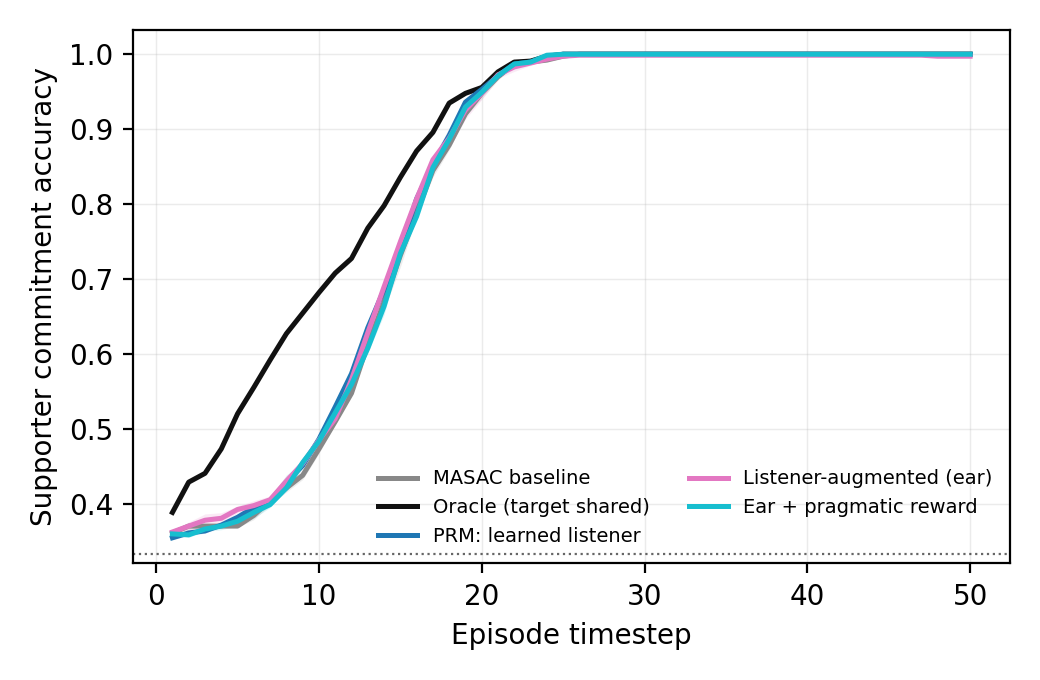
\includegraphics[width=0.95\columnwidth]{img/scout_commit_curve.png}
\caption{Supporter commitment accuracy over the episode (converged policies, 256 held-out episodes). All non-oracle conditions overlap: neither speaker-side rewards nor the deployed ear move the moment of understanding, because no condition produces first-leg signal for the ear to hear.}
\label{fig:commit_curve}
\end{figure}

\begin{figure}[t]
\centering
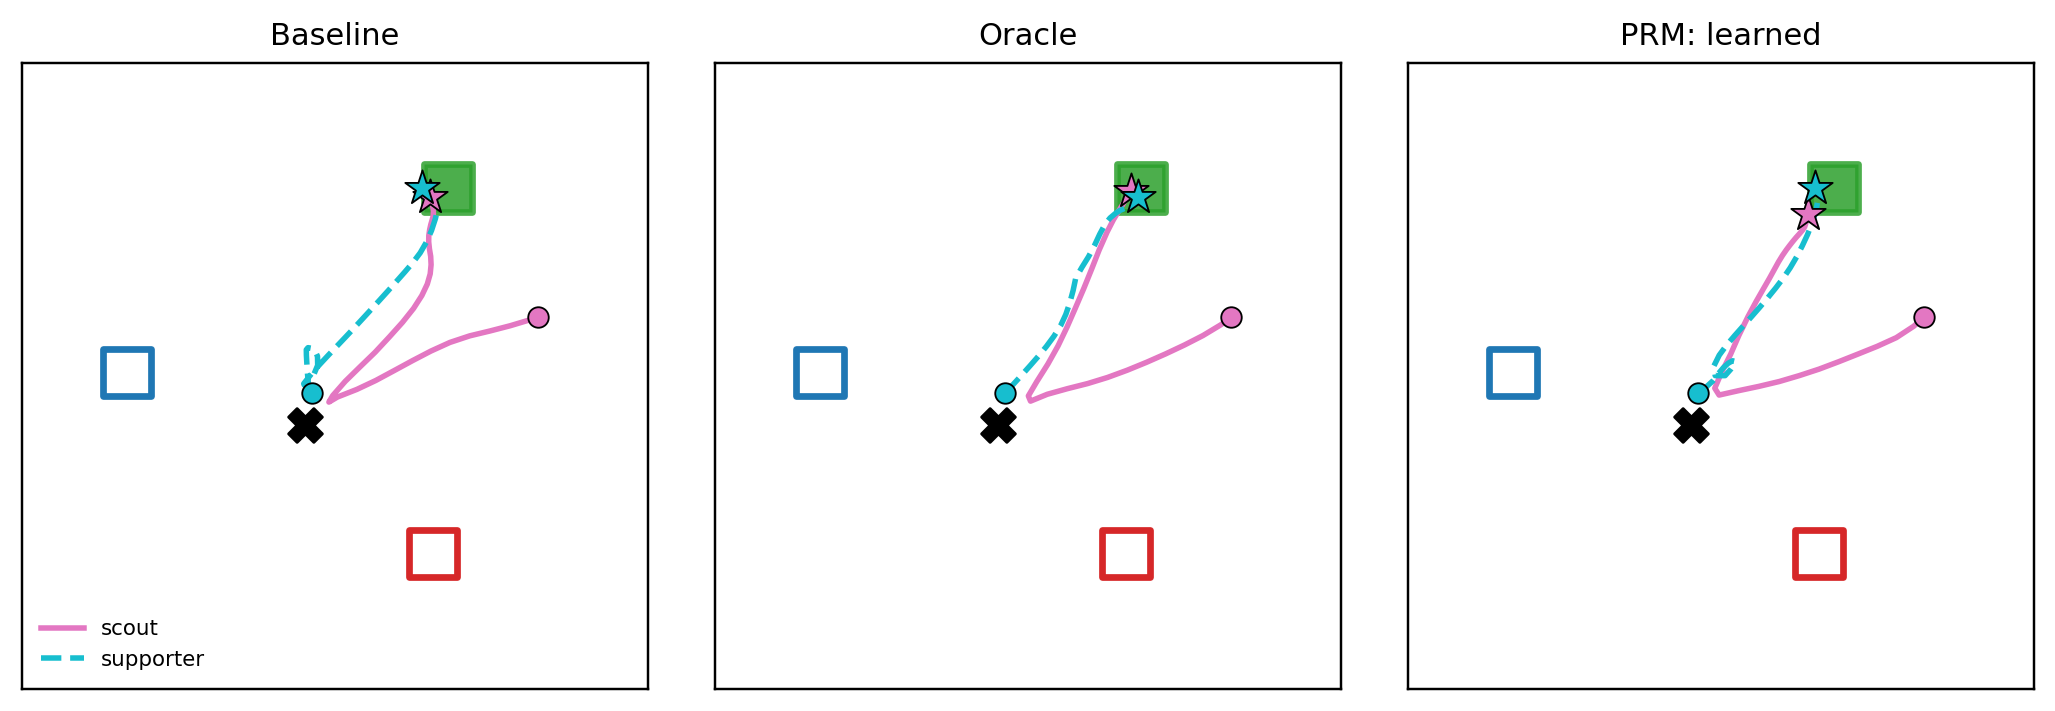
\includegraphics[width=\columnwidth]{img/scout_trajectories.png}
\caption{A held-out Environment A episode. Squares are sites (the true target filled), the cross is the pickup waypoint. Trajectories darken with time (dot every 5 steps; dense dots = slow motion): the baseline supporter hedges and corrects late, while informed supporters commit early. Open circle = start, star = end.}
\label{fig:scout_traj}
\end{figure}

\subsection{Environment B: The Cost of Signaling with Nothing to Say}
\label{ssec:results_spread}

Table~\ref{tab:final} summarizes final performance in the control environment; Figures~\ref{fig:task_reward}--\ref{fig:comm_reward} show training dynamics.

\begin{table}[t]
\centering
\caption{Final performance (mean $\pm$ s.e.m.\ over 3 seeds, averaged over the last three evaluations). $\Rext$ is the per-step team reward; Spec.\ is team specialization; $\Rcomm$ is each condition's own communicative reward (information-gain scale); Post-hoc is the decoding accuracy of a fresh listener trained on the final policy's rollouts (chance $=.33$).}
\label{tab:final}
\setlength{\tabcolsep}{3.0pt}
\begin{tabular}{lcccc}
\toprule
\textbf{Condition} & $\Rext$ & Spec. & $\Rcomm$ & Post-hoc \\
\midrule
Baseline & $1.07\pm.03$ & $.847$ & --- & $.598\pm.02$ \\
Oracle & $0.99\pm.04$ & $.841$ & --- & $.589\pm.01$ \\
\midrule
Simple $L_0$ & $0.93\pm.06$ & $.833$ & $-1.33$ & $.599\pm.01$ \\
Exclusivity $L_0$ & $0.57\pm.04$ & $.815$ & $-2.39$ & $.604\pm.02$ \\
\midrule
Learned $\Ltheta$ & $1.03\pm.08$ & $.847$ & $-0.13$ & $.582\pm.03$ \\
Learned + RSA & $\mathbf{1.09\pm.03}$ & $\mathbf{.853}$ & $\mathbf{-0.13}$ & $.578\pm.02$ \\
\bottomrule
\end{tabular}
\end{table}

\subsubsection{Hand-Crafted Listeners: Miscalibrated Signaling}
\label{ssec:results_heuristic}

The exclusivity listener exhibits an instructive failure mode, which we also observed in preliminary experiments with an independent, larger-scale implementation. The composite reward is clearly operative---early in training it even \emph{accelerates} learning (Fig.~\ref{fig:task_reward}), and it drives the geometric probe accuracy up faster than any other condition (Fig.~\ref{fig:probe_acc})---yet the agent never comes close to optimizing the communicative reward itself. $\Rcomm$ plateaus around $-2.4$ (Fig.~\ref{fig:comm_reward}), \emph{below} the uninformative level of zero: the pragmatic listener built on this common ground assigns the true meaning \emph{less} probability than a uniform guess. The exclusivity score (Eq.~\ref{eq:exclusivity}) demands that an action align with the true target's direction while misaligning with every competing direction; when landmarks subtend similar bearings this margin is geometrically unsatisfiable, so the agent pays a permanent tax for a signal that cannot be produced. The tax is visible everywhere: final task reward drops by $47\%$ relative to the baseline, distance and collision penalties rise, and specialization saturates lower ($.815$ vs.\ $.847$). The simple cosine listener, which removes the exclusivity margin, is correspondingly less harmful ($\Rext = 0.93$) and achieves a better---but still negative---$\Rcomm$. We call this failure mode \emph{miscalibrated signaling}: a hand-crafted common ground rewards behavior the policy cannot realize and an observer cannot decode, converting the intrinsic reward into pure interference.

\subsubsection{Learned Listeners: Calibrated Legibility}
\label{ssec:results_learned}

The learned listener changes the picture qualitatively. Both learned conditions steadily optimize their communicative reward from $-0.65$ toward zero (Fig.~\ref{fig:comm_reward}), confirming that the co-adapted reward is learnable---by construction, it only credits distinctions that are actually present in the behavioral distribution. This calibration eliminates the destructive interference: task performance is statistically indistinguishable from the baseline ($1.03\pm.08$ and $1.09\pm.03$ vs.\ $1.07\pm.03$), with the pragmatic variant nominally best on task reward and specialization. During training, the co-adapting listener's accuracy climbs from chance ($1/3$) to $\approx.43$ and is still rising at the end (Fig.~\ref{fig:listener_acc}), with the RSA-recursed variant consistently ahead of the purely literal one---suggesting that contrastive reasoning over alternatives extracts signal that maximum-likelihood decoding alone does not.

\subsubsection{How Much Was There to Say? Oracles and Post-Hoc Probes}
\label{ssec:results_oracle}

Two further measurements put the above in perspective. First, the oracle: giving agents their teammates' true preferences does \emph{not} improve task performance ($0.99$ vs.\ $1.07$). Near-optimal coordination in this environment is achievable from positions and velocities alone---who is closest to what resolves most conflicts---so the marginal task value of intent information is small. Second, the post-hoc probes: a fresh listener trained on any condition's \emph{converged} behavior decodes intentions at $.58$--$.60$ accuracy (Table~\ref{tab:final}), with no significant differences across conditions. Because acting on one's preference is extrinsically rewarded, converged behavior is already informative; at $\lambda=0.1$ there is simply little decodable information left for a calibrated reward to add---which the learned listener correctly reflects by saturating near zero, and which the hand-crafted listeners ignore by charging a permanent task tax for no informational return.

Together these results reframe the evaluation of implicit-communication methods: task reward alone conflates the cost of signaling with its value, and a method should be judged on (a) whether its intrinsic reward is achievable (calibration), (b) how much decodable information the resulting behavior carries (post-hoc probes), and (c) what it pays for that information (task-reward gap). On all three criteria the learned listener dominates the hand-crafted ones.

\subsubsection{The Weight $\lambda$: Dial or Landmine?}
\label{ssec:results_lambda}

We sweep the communicative weight for both listener families in Environment B (2 seeds per new point; Fig.~\ref{fig:lambda_ablation}). With the learned listener, $\lambda$ behaves like a dial along an information-performance frontier: $\lambda=0.1$ is free ($\Rext=1.03$, $\Rcomm=-0.13$); $\lambda=0.3$ buys near-saturated clarity ($\Rcomm=-0.05$) for a modest task cost ($\Rext=0.84$); and $\lambda=1.0$ pushes the communicative reward to genuinely \emph{positive} information gain ($\Rcomm=+0.62$)---behavior more informative than task-optimal motion---at a large task cost ($\Rext=-0.80$) as agents privilege signaling over covering landmarks. With the exclusivity listener, no operating point buys information: at $\lambda=0.03$ the reward is simply ignored ($\Rcomm$ stuck at $-2.6$, task performance at baseline level), and at $\lambda=0.1$ it destroys 47\% of task reward with $\Rcomm$ still at $-2.4$. Calibration is precisely what turns $\lambda$ from a landmine into a dial.

\begin{figure}[t]
\centering
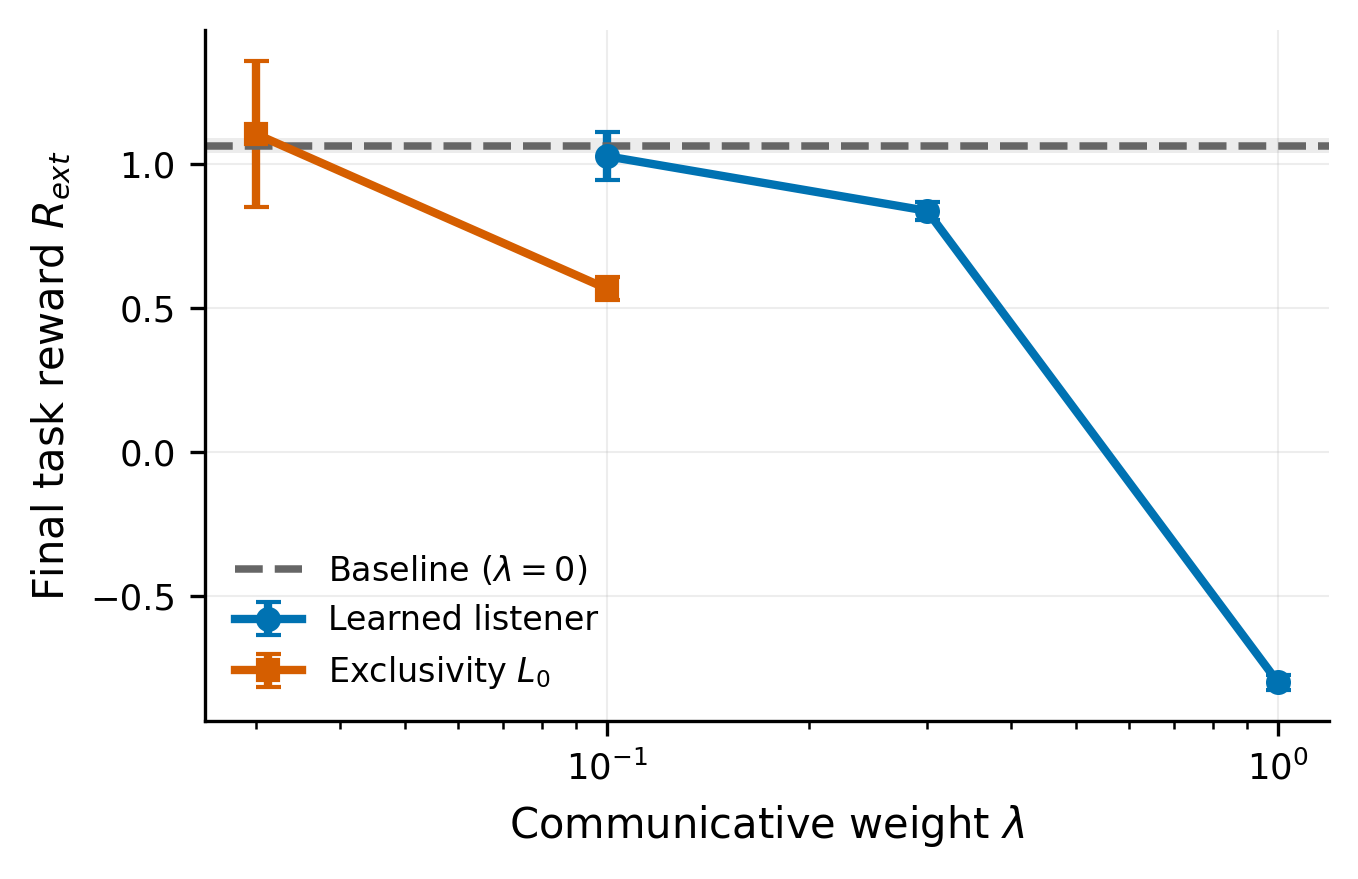
\includegraphics[width=0.9\columnwidth]{img/lambda_ablation.png}
\caption{Final task reward vs.\ communicative weight $\lambda$. The learned listener trades task reward for information smoothly; the exclusivity listener offers no $\lambda$ at which information is gained.}
\label{fig:lambda_ablation}
\end{figure}

\subsubsection{Qualitative Behavior}
\label{ssec:results_qualitative}

Figure~\ref{fig:trajectories} shows a representative held-out episode of Environment B. The baseline reaches landmarks but meanders, with late target switches. The exclusivity-listener agent displays the miscalibration diagnosed above: trajectories sweep across the arena and settle far from any landmark---costly motion signaling nothing. The learned-pragmatic agent produces direct, mutually distinct paths: each agent claims a separate landmark, and the agent whose preferred landmark is taken by a teammate cleanly re-targets the remaining one.

\begin{figure}[t]
\centering
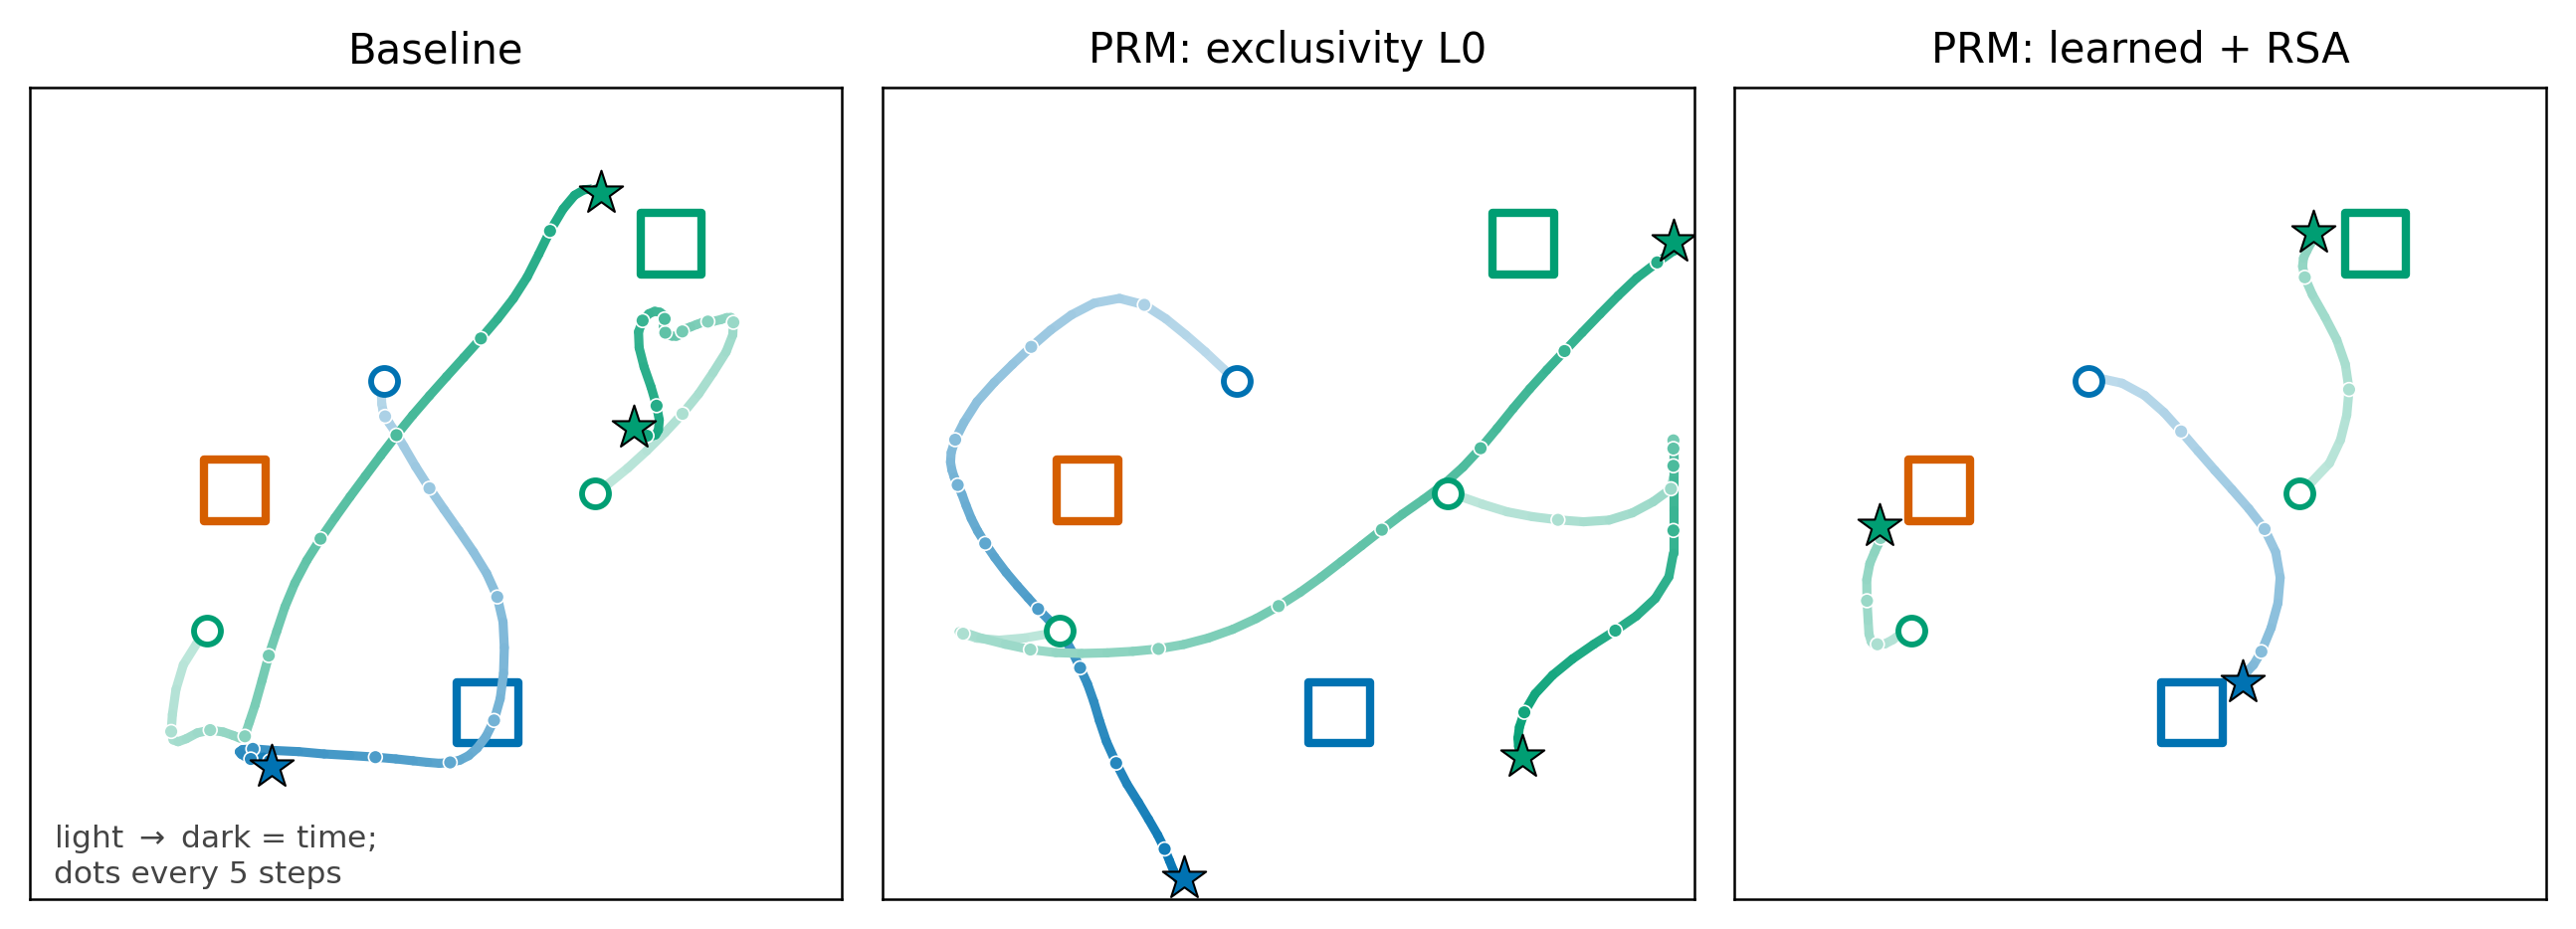
\includegraphics[width=\columnwidth]{img/trajectories.png}
\caption{A held-out episode under three conditions. Squares are landmarks (color = category); each trajectory is colored by the agent's \emph{private preference} and darkens with time, with a dot every 5 steps, so dense dots mean slow or stationary motion. Open circle = start, star = end.}
\label{fig:trajectories}
\end{figure}

\begin{figure}[t]
\centering
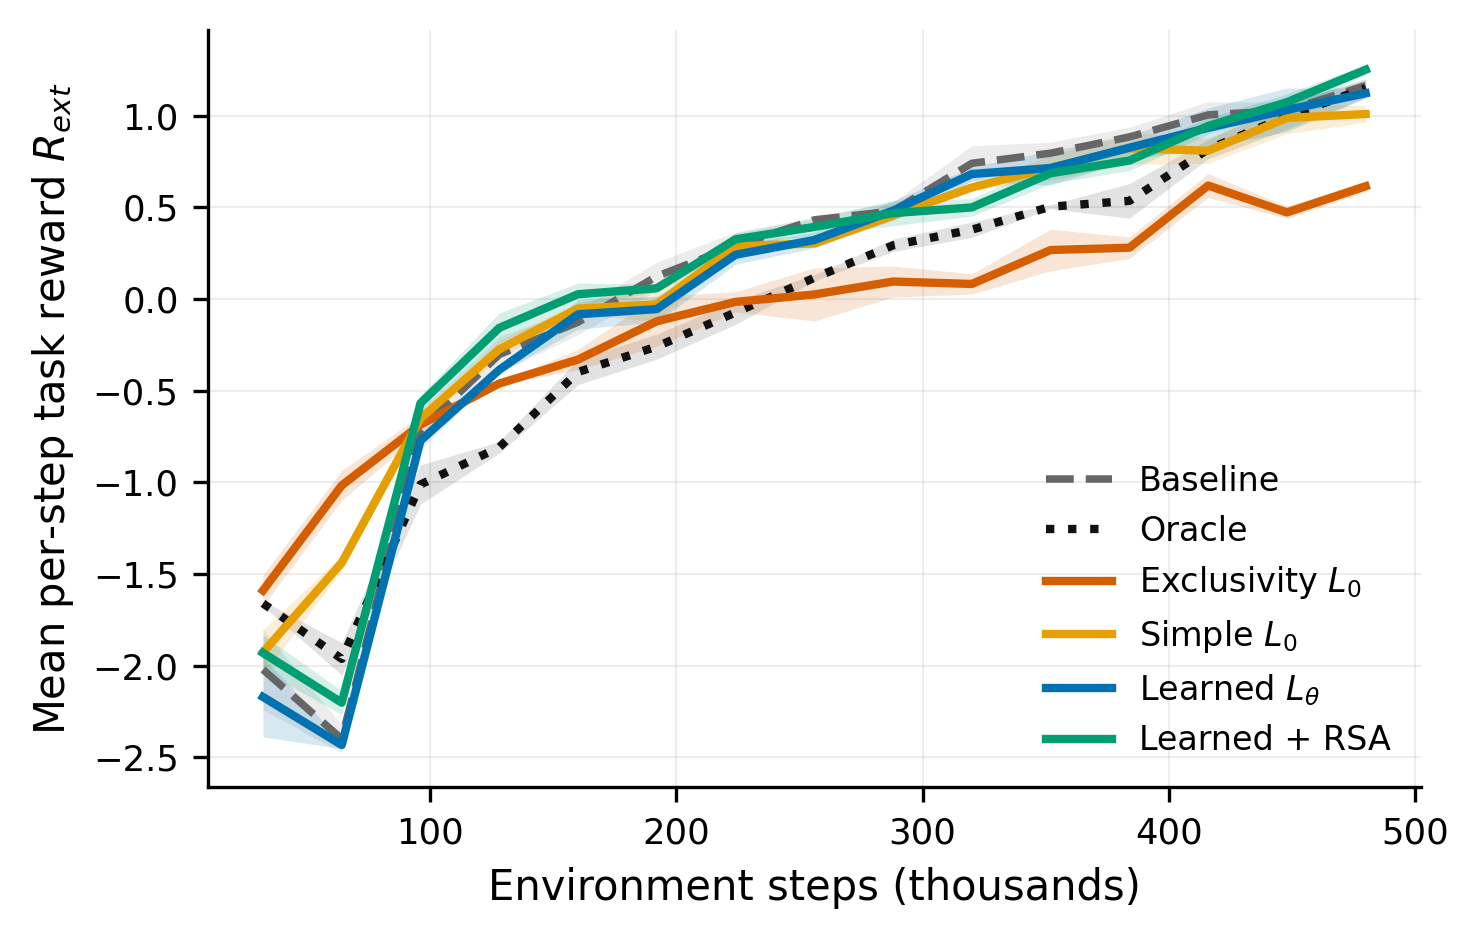
\includegraphics[width=0.93\columnwidth]{img/task_reward.png}
\caption{Mean per-step team reward $\Rext$ (3 seeds, mean $\pm$ s.e.m.).}
\label{fig:task_reward}
\end{figure}

\begin{figure}[t]
\centering
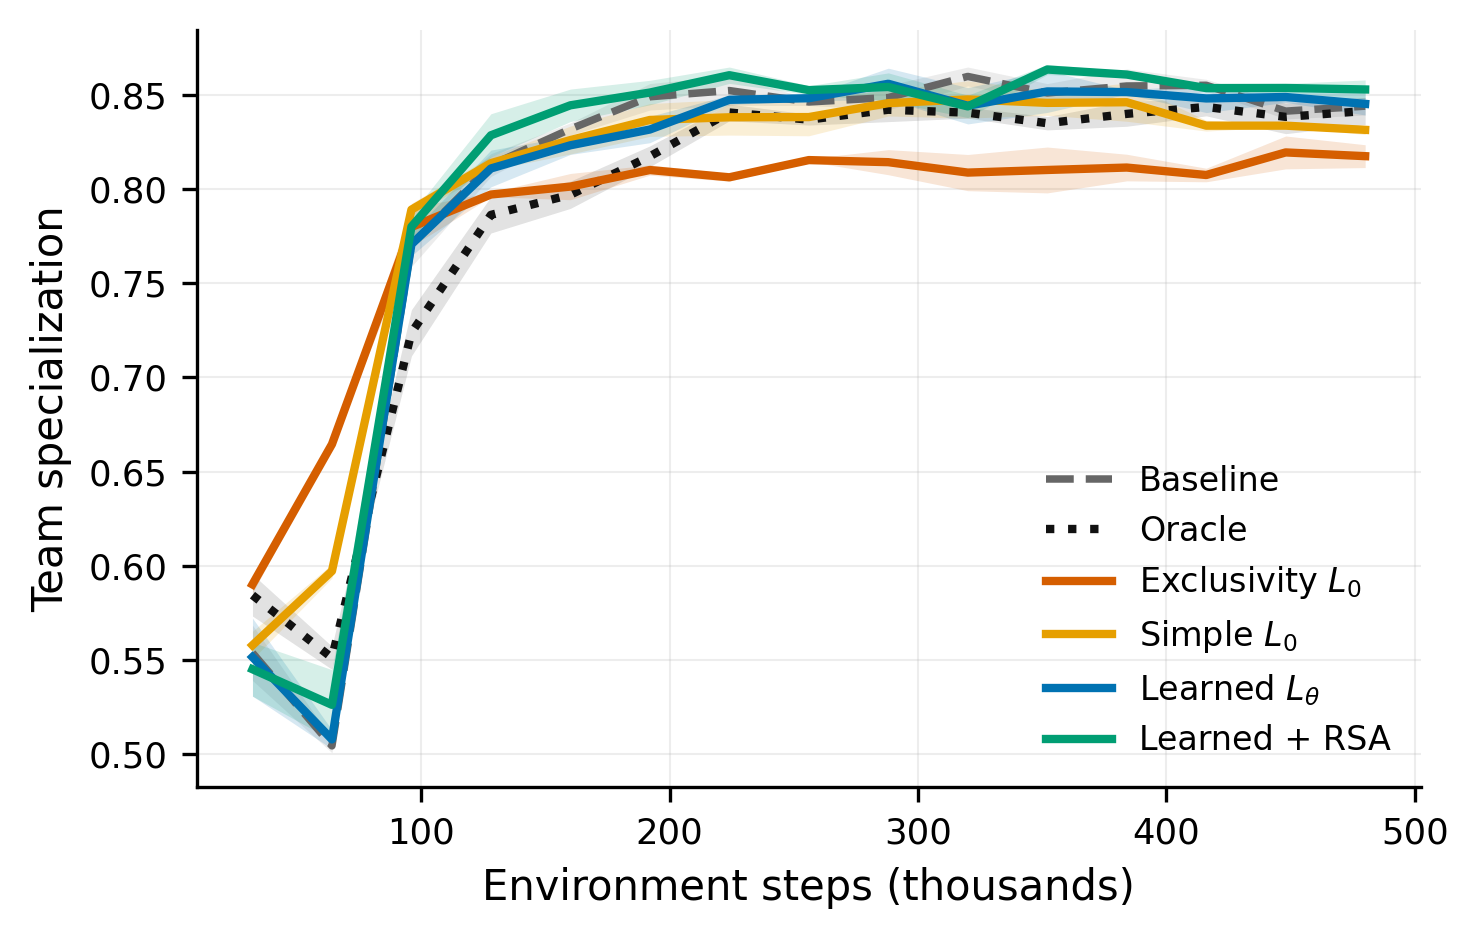
\includegraphics[width=0.93\columnwidth]{img/specialization.png}
\caption{Team specialization: fraction of landmarks claimed uniquely.}
\label{fig:specialization}
\end{figure}

\begin{figure}[t]
\centering
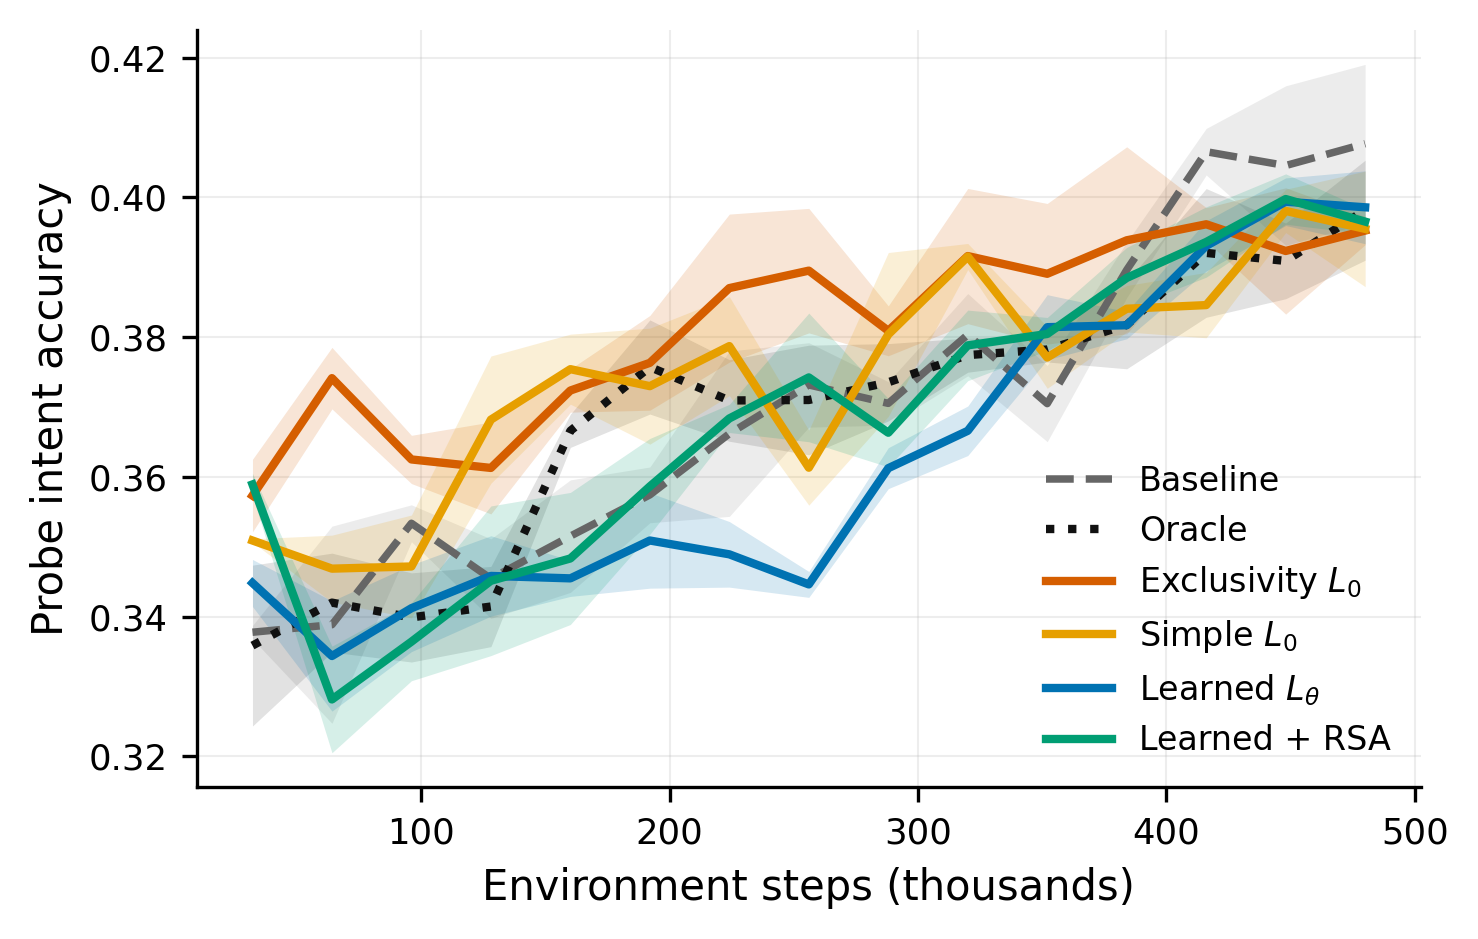
\includegraphics[width=0.93\columnwidth]{img/probe_acc.png}
\caption{Probe intent accuracy under the fixed geometric probe listener, identical across conditions.}
\label{fig:probe_acc}
\end{figure}

\begin{figure}[t]
\centering
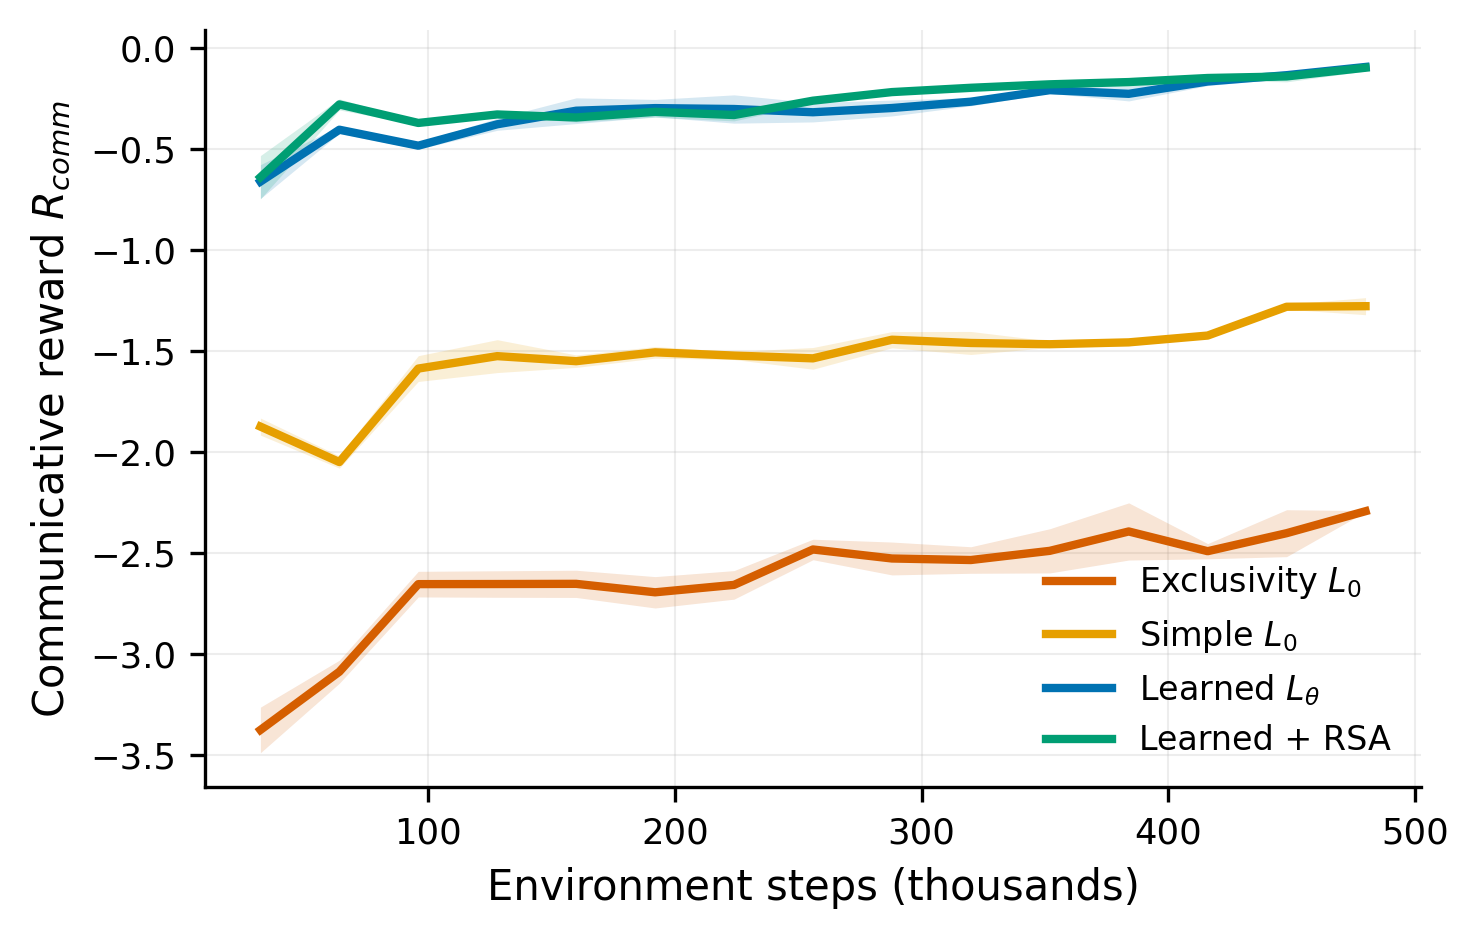
\includegraphics[width=0.93\columnwidth]{img/comm_reward.png}
\caption{Achieved communicative reward $\Rcomm$ (each condition under its own listener; information-gain scale, 0 = uninformative).}
\label{fig:comm_reward}
\end{figure}

\section{Discussion}
\label{sec:discussion}

\textbf{The common ground is the problem.} Our central empirical finding is that the success of a pragmatic reward hinges almost entirely on the alignment between the literal listener and the agents' realizable behavior. A hand-crafted $L_0$ encodes the designer's theory of what signaling should look like; when that theory is even mildly wrong---as with the exclusivity margin, which demands geometrically unsatisfiable action patterns---the recursion built on top of it faithfully amplifies the error, and the agent is paid to produce elaborate, undecodable gestures. This failure is quiet: behavioral metrics (path deviation, action magnitude, early probe accuracy) suggest the agent is ``signaling harder,'' while the communicative channel carries nothing. We suspect this failure mode is widespread in reward designs that score behavior against idealized observer models, and recommend a simple diagnostic that requires no extra machinery: track whether the agent can drive its own intrinsic reward above the uninformative level. A persistently negative information gain is a certificate of miscalibration.

\textbf{Learning the listener closes the loop.} Training $\Ltheta$ on the agents' own replay data guarantees that the common ground never demands what the policy distribution does not contain; the reward then only sharpens distinctions that already exist, which is why it optimizes smoothly and costs no task performance. Proposition~\ref{prop:mi} explains the mechanism: the learned-listener reward is a variational mutual-information bound, so policy improvement against it is information maximization---grounded, by construction, in a decodable channel. And because the bound is calibrated, its weight becomes meaningful: $\lambda$ moves the policy along an actual information-performance frontier (Sec.~\ref{ssec:results_lambda}) instead of scaling an arbitrary shaping term. The RSA recursion contributes during training: it consistently improves the co-adapting listener's accuracy, suggesting that pragmatic contrast (scoring an action against foregone alternatives) accelerates the emergence of decodable behavior, even where asymptotic decodability is capped by the task.

\textbf{Communication is a two-sided market.} Environment A decomposes implicit communication into its two halves and shows that rewarding either alone is insufficient. Speaker-side pragmatic rewards produce a decodable channel---the learned listener reads the scout at $92\%$---but a teammate trained by reward alone never learns to read it; receiver-side listener deployment provides the ear, but hears nothing during the window that matters because the unpressured speaker has nothing to say there. Each side's investment is worthless without the other's, a coordination equilibrium that mirrors the joint-exploration problem of emergent communication \cite{eccles2019biases} and, we suspect, explains why speaker-only legibility methods often show muted task gains.

\textbf{Clarity must be paid when it is needed.} The subsidy framing also exposes a subtler defect in legibility rewards as standardly defined, including ours: they integrate clarity uniformly over time. A rational speaker paid by the average sharpens the parts of its behavior that are cheapest to disambiguate---in our benchmark, the second leg, where motion already reveals the goal---and the channel stays silent exactly where the partner's decisions hang on it. Escalating $\lambda$ purchases more of the same lazy clarity at increasing task cost. The natural correction is to weight $\Rcomm$ by the \emph{partner's value of information}---clarity should be priced by what the listener can still do with it. Our filter listener, which compounds early evidence into every subsequent step's belief, is a hand-crafted step in this direction; a principled treatment would derive the weighting from the partner's counterfactual value function, which we leave to future work.
%%% DISCUSSION_LAMBDA_SLOT %%%

\textbf{When does legibility pay?} The contrast between environments is a caution for the field: in Environment B, where geometry resolves coordination, even a perfect oracle gains nothing, and a well-calibrated legibility reward correctly approaches a no-op; in Environment A the same machinery faces a certified $0.3$-per-step opportunity. Benchmarks for communicative MARL should report their oracle gap---without it, task reward conflates the cost of signaling with its value. Where the gap is large, our results argue for evaluating methods on three separable axes: calibration of the intrinsic reward, information actually transmitted (probes and deployed listeners), and the task price paid for it.

\subsection{Limitations and Future Work}
\label{ssec:limitations}

Several limitations qualify our findings and chart future work. First, the intrinsic reward densifies the learning signal, which can aid learning independently of legibility; our commitment-timing and probe metrics mitigate but do not eliminate this confound. Second, our negative receiver-side results are claims about a training budget and architecture (feed-forward policies, 480k steps), not impossibility results; recurrent supporters, longer training, or curricula might crack the joint-exploration equilibrium that our budget did not. Third, meanings are hand-specified discrete variables; extending $\Rcomm$ to continuous, hierarchical, or self-assigned meaning spaces---where the agent learns \emph{what} is worth communicating, not only how---remains open. Fourth, validation is confined to AI-AI teams in 2D particle worlds; whether computational legibility transfers to \emph{human-perceived} legibility must be established with human observers, for instance by fitting $\Ltheta$ to human intent judgments. Finally, the framework is symmetric in an intriguing way: inverting the sign of $\lambda$ turns legibility into \emph{obfuscation}, suggesting privacy-preserving applications where agents remain opaque to opponents while staying legible to allies \cite{strouse2018learning}.

\section{Conclusion}
\label{sec:conclusion}

We presented a framework that unifies pragmatic inference and maximum-entropy reinforcement learning, importing the RSA listener value as a principled intrinsic reward for legible behavior, with the literal listener---the assumed common ground---as its decisive design choice; learning that listener jointly with the policy aligns the reward with what observers can actually decode and recovers information-theoretic approaches as a special case. Our two-environment study then locates the real obstacles. Where communication has no task value, miscalibrated hand-crafted listeners charge for undecodable signaling while calibrated ones correctly approach a no-op. Where communication is certifiably valuable, speaker-side rewards make behavior decodable but cannot make a teammate listen; deploying the learned listener as the teammate's ear recovers part of the oracle gap; and what remains is a two-sided equilibrium sustained by uniformly-integrated clarity rewards that pay for clarity where it is cheap rather than when it is needed. The path forward for pragmatic agents, we argue, runs through value-weighted clarity and joint speaker-listener training---toward agents whose competence includes being understood, exactly when being understood matters.

\vfill\pagebreak

\appendix
\section{Hyperparameters}
\begin{table}[h]
\centering
\caption{Hyperparameters (all conditions unless noted).}
\label{tab:hyperparams}
\begin{tabular}{ll}
\toprule
\textbf{Parameter} & \textbf{Value} \\
\midrule
Parallel environments & 64 \\
Episode length & 50 \\
Total environment steps & 480k \\
Actor / critic architecture & MLP $256\times256$ \\
Learning rate (actor, critic) & $3\times10^{-4}$ \\
Discount $\gamma$ & 0.95 \\
Target smoothing $\tau$ & 0.005 \\
Batch size / updates per env step & 512 / 4 \\
Entropy target & $-\dim(\mathcal{A})$ (auto-tuned) \\
$\lambda$ (pragmatic weight) & 0.1 \\
Listener $\Ltheta$ & MLP $128\times128$, lr $10^{-3}$ \\
Heuristic listener temp.\ $\alpha_{\text{temp}}$ / $K$ / $N_r$ & 5 / 64 / 1 \\
Learned+RSA alternatives / $N_r$ & 16 / 1 \\
Filter listener temp.\ / forgetting $\rho$ & 2 / 0.9 \\
Scout / supporter max speed (Env.\ A) & 1.0 / 0.6 \\
Rendezvous bonus / cover radius (Env.\ A) & 3.0 / 0.3 \\
Seeds per condition & 3 \\
\bottomrule
\end{tabular}
\end{table}

% References
% -------------------------------------------------------------------------
\bibliographystyle{IEEEbib}

\begin{thebibliography}{10}

\bibitem{dragan2013legibility}
Anca~D. Dragan, Kenton~C.T. Lee, and Siddhartha~S. Srinivasa,
\newblock ``Legibility and predictability of robot motion,''
\newblock in {\em ACM/IEEE International Conference on Human-Robot Interaction (HRI)}, 2013, pp. 301--308.

\bibitem{goodman2016pragmatic}
Noah~D. Goodman and Michael~C. Frank,
\newblock ``Pragmatic language interpretation as probabilistic inference,''
\newblock {\em Trends in Cognitive Sciences}, vol. 20, no. 11, pp. 818--829, 2016.

\bibitem{estienne2025collaborative}
Lautaro Estienne, Gabriel Ben~Zenou, Nona Naderi, Jackie~Chi~Kit Cheung, and Pablo Piantanida,
\newblock ``Collaborative rational speech act: Pragmatic reasoning for multi-turn dialog,''
\newblock in {\em Proceedings of the 2025 Conference on Empirical Methods in Natural Language Processing (EMNLP)}, 2025.

\bibitem{strouse2018learning}
DJ~Strouse, Max Kleiman-Weiner, Josh Tenenbaum, Matt Botvinick, and David~J. Schwab,
\newblock ``Learning to share and hide intentions using information regularization,''
\newblock in {\em Advances in Neural Information Processing Systems}, 2018, vol.~31.

\bibitem{eysenbach2019diversity}
Benjamin Eysenbach, Abhishek Gupta, Julian Ibarz, and Sergey Levine,
\newblock ``Diversity is all you need: Learning skills without a reward function,''
\newblock in {\em International Conference on Learning Representations}, 2019.

\bibitem{ziebart2008maximum}
Brian~D. Ziebart, Andrew~L. Maas, J.~Andrew Bagnell, and Anind~K. Dey,
\newblock ``Maximum entropy inverse reinforcement learning,''
\newblock in {\em Proceedings of the AAAI Conference on Artificial Intelligence}, 2008, pp. 1433--1438.

\bibitem{baker2017rational}
Chris~L. Baker, Julian Jara-Ettinger, Rebecca Saxe, and Joshua~B. Tenenbaum,
\newblock ``Rational quantitative attribution of beliefs, desires and percepts in human mentalizing,''
\newblock {\em Nature Human Behaviour}, vol. 1, no. 4, pp. 0064, 2017.

\bibitem{rabinowitz2018machine}
Neil~C. Rabinowitz, Frank Perbet, H.~Francis Song, Chiyuan Zhang, S.M.~Ali Eslami, and Matthew Botvinick,
\newblock ``Machine theory of mind,''
\newblock in {\em International Conference on Machine Learning}, 2018, pp. 4218--4227.

\bibitem{faria2024guess}
Miguel Faria, Francisco~S. Melo, and Ana Paiva,
\newblock ``\,``Guess what I'm doing'': Extending legibility to sequential decision tasks,''
\newblock {\em Artificial Intelligence}, vol. 330, pp. 104107, 2024.

\bibitem{miura2021unifying}
Shuwa Miura and Shlomo Zilberstein,
\newblock ``A unifying framework for observer-aware planning and its complexity,''
\newblock in {\em Conference on Uncertainty in Artificial Intelligence (UAI)}, 2021, pp. 610--620.

\bibitem{miura2024observer}
Shuwa Miura and Shlomo Zilberstein,
\newblock ``Observer-aware planning with implicit and explicit communication,''
\newblock in {\em International Conference on Autonomous Agents and Multiagent Systems (AAMAS)}, 2024, pp. 1409--1417.

\bibitem{liu2025active}
Yanyu Liu, Yinghui Pan, Yifeng Zeng, Biyang Ma, and Prashant Doshi,
\newblock ``Active legibility in multiagent reinforcement learning,''
\newblock {\em Artificial Intelligence}, vol. 346, pp. 104357, 2025.

\bibitem{oguntola2023theory}
Ini Oguntola, Joseph Campbell, Simon Stepputtis, and Katia Sycara,
\newblock ``Theory of mind as intrinsic motivation for multi-agent reinforcement learning,''
\newblock in {\em ICML Workshop on Theory of Mind in Communicating Agents}, 2023.

\bibitem{jaques2019social}
Natasha Jaques, Angeliki Lazaridou, Edward Hughes, Caglar Gulcehre, Pedro~A. Ortega, DJ~Strouse, Joel~Z. Leibo, and Nando de~Freitas,
\newblock ``Social influence as intrinsic motivation for multi-agent deep reinforcement learning,''
\newblock in {\em International Conference on Machine Learning}, 2019, pp. 3040--3049.

\bibitem{eccles2019biases}
Tom Eccles, Yoram Bachrach, Guy Lever, Angeliki Lazaridou, and Thore Graepel,
\newblock ``Biases for emergent communication in multi-agent reinforcement learning,''
\newblock in {\em Advances in Neural Information Processing Systems}, 2019, vol.~32.

\bibitem{bard}
Jakob~N. Foerster, Francis Song, Edward Hughes, Neil Burch, Iain Dunning, Shimon Whiteson, Matthew Botvinick, and Michael Bowling,
\newblock ``Bayesian action decoder for deep multi-agent reinforcement learning,''
\newblock in {\em International Conference on Machine Learning}, 2019, pp. 1942--1951.

\bibitem{sad}
Hengyuan Hu and Jakob~N. Foerster,
\newblock ``Simplified action decoder for deep multi-agent reinforcement learning,''
\newblock in {\em International Conference on Learning Representations}, 2020.

\bibitem{obl}
Hengyuan Hu, Adam Lerer, Brandon Cui, Luis Pineda, Noam Brown, and Jakob Foerster,
\newblock ``Off-belief learning,''
\newblock in {\em International Conference on Machine Learning}, 2021, pp. 4369--4379.

\bibitem{foerster2016learning}
Jakob Foerster, Ioannis~Alexandros Assael, Nando de~Freitas, and Shimon Whiteson,
\newblock ``Learning to communicate with deep multi-agent reinforcement learning,''
\newblock in {\em Advances in Neural Information Processing Systems}, 2016, vol.~29.

\bibitem{sukhbaatar2016learning}
Sainbayar Sukhbaatar, Arthur Szlam, and Rob Fergus,
\newblock ``Learning multiagent communication with backpropagation,''
\newblock in {\em Advances in Neural Information Processing Systems}, 2016, vol.~29.

\bibitem{boldt2024review}
Brendon Boldt and David Mortensen,
\newblock ``A review of the applications of deep learning-based emergent communication,''
\newblock {\em Transactions on Machine Learning Research}, 2024.

\bibitem{zaslavsky2021rate}
Noga Zaslavsky, Jennifer Hu, and Roger~P. Levy,
\newblock ``A rate-distortion view of human pragmatic reasoning,''
\newblock in {\em Proceedings of the Society for Computation in Linguistics}, 2021, pp. 347--348.

\bibitem{andreas2016reasoning}
Jacob Andreas and Dan Klein,
\newblock ``Reasoning about pragmatics with neural listeners and speakers,''
\newblock in {\em Proceedings of the 2016 Conference on Empirical Methods in Natural Language Processing (EMNLP)}, 2016, pp. 1173--1182.

\bibitem{fried2018unified}
Daniel Fried, Jacob Andreas, and Dan Klein,
\newblock ``Unified pragmatic models for generating and following instructions,''
\newblock in {\em Proceedings of NAACL-HLT}, 2018, pp. 1951--1963.

\bibitem{haarnoja2018soft}
Tuomas Haarnoja, Aurick Zhou, Pieter Abbeel, and Sergey Levine,
\newblock ``Soft actor-critic: Off-policy maximum entropy deep reinforcement learning with a stochastic actor,''
\newblock in {\em International Conference on Machine Learning}, 2018, pp. 1861--1870.

\bibitem{levine2018reinforcement}
Sergey Levine,
\newblock ``Reinforcement learning and control as probabilistic inference: Tutorial and review,''
\newblock {\em arXiv preprint arXiv:1805.00909}, 2018.

\bibitem{barber2003im}
David Barber and Felix Agakov,
\newblock ``The IM algorithm: A variational approach to information maximization,''
\newblock in {\em Advances in Neural Information Processing Systems}, 2003, vol.~16.

\bibitem{lowe2017multi}
Ryan Lowe, Yi~Wu, Aviv Tamar, Jean Harb, Pieter Abbeel, and Igor Mordatch,
\newblock ``Multi-agent actor-critic for mixed cooperative-competitive environments,''
\newblock in {\em Advances in Neural Information Processing Systems}, 2017, vol.~30.

\end{thebibliography}

\end{document}
